\documentclass{article}
% translate with >> pdflatex -shell-escape <file>

% This file is used as unit test for pgfplots, copyright by Christian Feuersaenger.
% 
% See
%   http://pgfplots.sourceforge.net/pgfplots.pdf
% for pgfplots.
%
% Any required input files (for <plot table> or <plot file> or the table package) can be downloaded
% at
% http://www.ctan.org/tex-archive/graphics/pgf/contrib/pgfplots/doc/latex/
% and
% http://www.ctan.org/tex-archive/graphics/pgf/contrib/pgfplots/doc/latex/plotdata/

\usepackage{pgfplots}
\pgfplotsset{compat=newest}

\pagestyle{empty}

\usepgfplotslibrary{smithchart}

\begin{document}


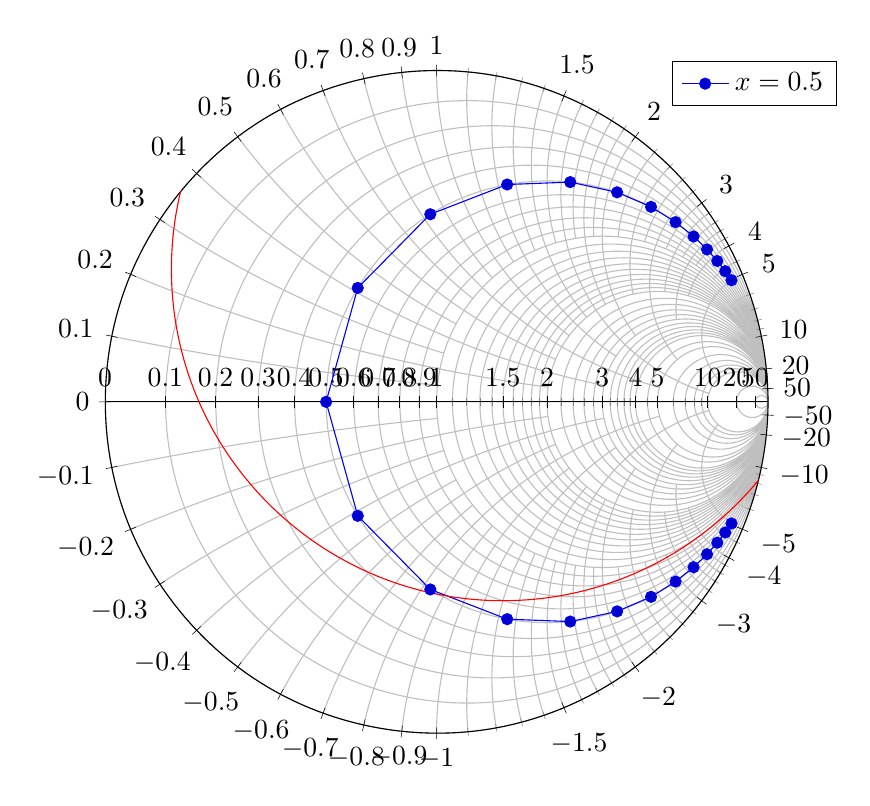
\begin{tikzpicture}
%\tracingmacros=2 \tracingcommands=2
	\begin{smithchartaxis}[
		width=10cm,
		height=10cm,
		xmin=0,xmax=50,
		ymin=-50,ymax=50,
		xtick={
			0,0.1,0.2,...,1,1.5,2,3,4,5,10,20,50%
		},
		ytick={%
			0,%
			0.1,0.2,...,1,1.5,2,3,4,5,10,20,50,%
			-0.1,-0.2,...,-1,-1.5,-2,-3,-4,-5,-10,-20,-50%
		},
		minor xtick={1.1,1.2,1.3,1.4,1.6,1.7,1.8,1.9,2.2,2.4,2.6,2.8,3.2,3.4,3.6,3.8,4.5,6,7,8,9},
		minor ytick={%
			1.1,1.2,1.3,1.4,1.6,1.7,1.8,1.9,2.2,2.4,2.6,2.8,3.2,3.4,3.6,3.8,4.5,6,7,8,9,%
			-1.1,-1.2,-1.3,-1.4,-1.6,-1.7,-1.8,-1.9,-2.2,-2.4,-2.6,-2.8,-3.2,-3.4,-3.6,-3.8,-4.5,-6,-7,-8,-9%
		},
		ygrid each nth passes x={1,2,3,5,10:3,20:3},
		%xtick={0,30,...,360},
	]
	\addplot+[domain=-5:5] (0.5,\x);
	\addlegendentry{$x=0.5$}
	\pgfplotsextra{%
		\draw[red] (1,1) circle (\pgfplotspointxaxislength/2);
	}
	\end{smithchartaxis}
\end{tikzpicture}
\end{document}
